Mobile devices in daily life are equipped with increasingly powerful computing and storage abilities, which enables individual devices to accumulate enormous valuable information. It facilitates a huge number of rising technologies such as edge computing and smart home. Meanwhile, the accumulated data in users' devices can be used to train models for various practical purposes due to the flourishing of machine learning. In traditional machine learning frameworks, data needs to be gathered into a central server in order to execute the learning process. However, most data collected by mobile devices is sensitive. Users usually refuse to send their private data to others, such as a learning center. This phenomenon impedes the development of distributed learning among common users.

Since the computing ability of mobile devices is powerful enough to run small-scale machine learning tasks, FL~\cite{mcmahan2016communicationefficient}, which is a distributed machine learning framework, becomes possible. FL's main purpose is to address the privacy problem in learning tasks and it is developing rapidly with increasing number of applications. For example, Google's keyboard query suggestions~\cite{yang2018applied} project was an effective application of FL. It trained a model that can predict users' input precisely without uploading users' private data. Figure~\ref{fed} illustrates the structure of FL. Parties receive a global model from the server and train their models based on their own data respectively. Afterwards, each party sends the parameters of their models to the server while the server runs a particular aggregation algorithm to compute the global model based on these parameters. In such frameworks, users do not need to send their data to the learning server, and thus the privacy of participants is to some extent protected.

Though FL can protect users' data, attackers can still eavesdrop a party's parameter during training process and then establish inference attacks~\cite{Beyond, Leakage, Nasr19} to reveal users' training data. Leaking these private data may cause severe consequence: if a hospital's diagnostic model is compromised, the patients' private medical-related information will be exposed, and this could result in potentially serious consequences. Additionally, as the server is provided by an untrusted third party, the untrusted party can easily obtain all participants' parameters in the aggregation process and conduct attacks. It is because that in the conventional FL framework~\cite{Nasr19}, parameters are directly sent to the server, and this enables the server to gather all information easily. Therefore, sending parameters to the server directly faces the threat of inference attacks. This kind of attack is quite severe as it can be established by any malicious or untrusted participant in the FL process. Therefore, how to conduct joint learning without leaking parameters to others comes into focus.

To tackle the privacy problem in FL, researchers proposed numerous secure aggregation protocols~\cite{shi2011privacy,RobustAgg,Bonawitz19,Nike,PrivFL} based on cryptography or other techniques. These protocols enable a group of parties who have private information to compute a function of these private data without revealing them. Therefore, employing secure aggregation in FL can help to protect models' intermediate parameters from being known by others. However, current solutions still have some shortcomings and deficiencies. A trivial solution is to employ homomorphic encryption (HE) to implement secure aggregation, Shi \emph{et al}.~\cite{shi2011privacy} utilized HE methods to achieve secure addition in FL. With the data encrypted, attackers cannot obtain any useful information from leaked messages. However, HE algorithms suffer from low efficiency which is hardly acceptable in FL~\cite{HESurvey}. Differential Privacy (DP) is another feasible method to implement secure aggregation. DP-based frameworks add noises to the parameters in order to deceive the attackers. The problem is that these noises also have an influence on the learning result~\cite{DLwDP}, therefore, there remains a tradeoff problem between the performance and security levels for DP methods in FL. What's more, the effects of DP-based methods are barely satisfactory~\cite{Bargav19}. Blockchain-based methods~\cite{DeepChain,Lu2020,On-Device} are also promising and provide high security, yet blockchain-based methods are still inefficient and implement-unfriendly so far.

\begin{figure}[!ht]
    \centering
    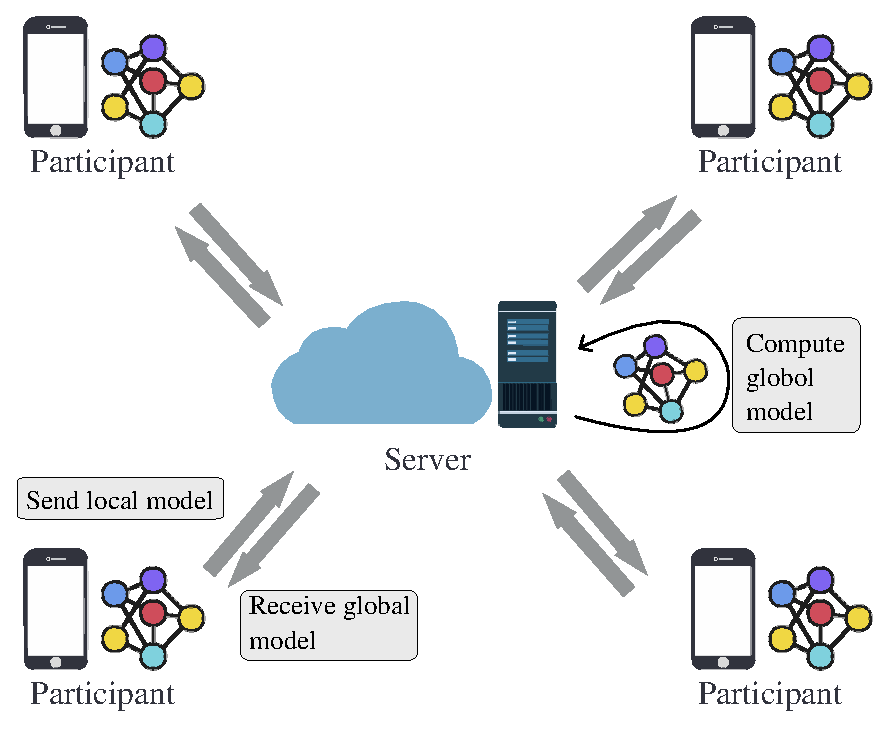
\includegraphics[width=0.9\columnwidth]{img/fed.eps}
    \caption{The structure of FL. Participants train local models respectively and send their parameters to the server for aggregation. The server compute the new global model based on received parameters and sends it to participants. This process usually will be repeated numerous times.}
    \label{fed}
\end{figure}

One may think that the multi-party computation (MPC)~\cite{Yao} technique can be leveraged to implement secure aggregation directly. However, most MPC protocols rely on the prerequisite that all participants are able to communicate with each other. In practice, participants of an FL task are unknown to each other, which means one party cannot communicate with another directly. This is a severe obstacle that prevents implementing MPC in FL. Bonawitz \emph{et al}.~\cite{Practical} utilized Diffie-Hellman key exchange to generate pairwise secret masks, however, this method has a dissatisfactory efficiency. The high communication overhead within MPC demands a prompt solution. A recent work~\cite{Two-Phase} also analyzed the MPC process in FL and tried to reduce the overheads by introducing a scheme named ``aggregation committee'', yet this method still has a high price on set-up. In addition, Bonawitz's work also pointed out that the robustness of FL frameworks is also significant because most MPC protocols will fail if there are some participants dropping out, and it usually costs a lot to recover from situations where several nodes are dropping out or crashed. In practice, mobile devices' communications are usually not stable enough, therefore, breakdowns and delays take places quite frequently. In summary, employing traditional MPC methods in a system with a large number of users is faced with a problem with efficiency and instability.

\subsection{Motivation} 
Prior works suffer from low efficiency, reducing accuracy or complex structures. Therefore, a secure, efficient and implement-friendly FL framework is desired. We aim to design an FL framework that:
\begin{enumerate}
    \item protects users' privacy by employing cryptography techniques while solving the problem that participants are unknown to each other.

    \item has a low communication overhead, avoiding constructing overmuch pairwise connections.

    \item is secure under semi-honest environments, where all users and the server may eavesdrop information.

    \item has high robustness with capability to handle emergencies where several participants may lose connection.

    \item has no negative influence on the quality of the trained model.
\end{enumerate}

\subsection{Our contribution}
\begin{enumerate}
    \item We propose Democratic Federated Learning (DemoFL), a novel FL framework that protects users' privacy with very low overhead. DemoFL employs a smart additive secret sharing protocol to realize MPC, which helps to hide intermediate parameters.

    \item DemoFL utilizes a hierarchical structure design to reduce the communication demands and improve the efficiency. It has a low time complexity as $O(n)$.

    \item We designed a consensus scheme to achieve ``democracy'' and high robustness. The consensus scheme helps to handle unexpected situations where a leader node or a common user is crashed. It selects leaders from all clients democratically and rapidly when such situations happen.

    \item We conduct a series of experiments and verified that DemoFL has satisfactory efficiency and robustness without reducing accuracy.

\end{enumerate}

\subsection{Roadmap} In Section~\ref{sec:back} we introduce the background and some definitions. Next, we introduce related work and some platforms of FL in Section~\ref{sec:related}. Section~\ref{sec:DemoFL} detailedly illustrates our proposed framework including the attack model. Evaluations for efficiency and security are stated in Section~\ref{sec:eval}, followed with experimental results in Section~\ref{sec:exp}. Finally, we give the conclusion and future expectations in Section~\ref{sec:conc}.